\ifx\boi\undefined\ifx\problemname\undefined
\providecommand\sampleinputname{}
\providecommand\sampleoutputname{}
\documentclass[lithuanian]{templates/boi}
\usepackage[L7x]{fontenc}
\problemlanguage{.lt}
\fi
\newcommand{\boi}{Baltijos šalių informatikos olimpiada}
\newcommand{\practicesession}{Bandomasis turas}
\newcommand{\contestdates}{2018 m. balandžio 27 - gegužės 1 d.}
\newcommand{\dayone}{1 diena}
\newcommand{\daytwo}{2 diena}
\newcommand{\licensingtext}{This problem is licensed under CC BY-SA 4.0.}
\newcommand{\problem}{Uždavinys}
\newcommand{\inputsection}{Pradiniai duomenys}
\newcommand{\outputsection}{Rezultatai}
\newcommand{\interactivity}{Realizacija}
\newcommand{\grading}{Vertinimas(?)}
\newcommand{\scoring}{Taškų skyrimas(?)}
\newcommand{\constraints}{Ribojimai}
\renewcommand{\sampleinputname}{Pradiniai duomenys}
\renewcommand{\sampleoutputname}{Rezultatai}
\newcommand{\sampleexplanation}[1]{Pirmojo pavyzdžio paaiškinimas}
\newcommand{\sampleexplanations}{Pavyzdžių paaiškinimai}
\newcommand{\timelimit}{Laiko ribojimas}
\newcommand{\memorylimit}{Atminties ribojimas}
\newcommand{\seconds}{s}
\newcommand{\megabytes}{MB}
\newcommand{\group}{Grupė}
\newcommand{\points}{Taškai}
\newcommand{\limitsname}{Ribojimai}
\newcommand{\additionalconstraints}{Papildomi ribojimai}
\newcommand{\testgroups}{
Jūsų sprendimas bus testuojamas su keliomis testų grupėmis, kiekviena kurių vertinama tam tikru skaičiumi taškų.
Kiekvieną testų grupę sudarys keletas testų.
Taškai už testų grupę skiriami tik jei įveikiate visus tos grupės testus.
}
\fi
\def\version{jury-1}
\problemname{Meilės daugiakampis}
Muilo operose dažnai yra daug veikėjų ir jų tarpusavio santykiai būna painūs.
Viename TV šou yra $N$ dalyvių. Kiekvienas dalyvis yra įsimylėjęs lygiai vieną dalyvį (gali būti įsimylėjęs ir save patį). Sakysime, kad du dalyviai yra užmezgę santykius, tada ir tik tada, kai jie vienas kitą įsimylėję.

Deja, tokia galimybė leidžia susidaryti sudėtingiems santykiams, kuriuos pavadinsime „meilės daugiakampiu“. Sakysime, kad 3 ar daugiau dalyvių priklauso „meilės daugiakampiui“, jei pirmasis įsimylėjo antrąjį, antrasis -- trečiąjį, ir t.t., o paskutinysis įsimylėjo pirmąjį.

Pastarosios apklausos parodė, kad žiūrovai pavargo nuo tokių dramų ir norėtų ko nors romantiškesnio. Todėl buvo nuspręsta į kai kuriuos dalyvius paleisti meilės strėles taip, kad kiekvienas dalyvis būtų užmezgęs santykius. Iššaudami meilės strėlę į dalyvį, galite pakeisti jo įsimylėjimo objektą (į bet kurį jūsų pasirinktą).

Kokį mažiausią skaičių strėlių reiktų paleisti, kad visi dalyviai būtų užmezgę santykius?

\section*{\inputsection}
Pirmoje eilutėje pateiktas sveikasis skaičius $N$ -- dalyvių skaičius.
Tolesnėse $N$ eilučių yra po du tarpu atskirtus vardus $s$ ir $t$, reiškiančius, kad dalyvis 
$s$ pradiniu momentu įsimylėjęs dalyvį $t$. Dalyvių vardų ilgiai neviršija $10$ simbolių ir sudaryti iš mažųjų anglų k. abėcėlės raidžių.

\section*{\outputsection}
Išveskite vieną sveikąjį skaičių -- mažiausią galimą meilės strėlių skaičių, kurias paleidus į dalyvius, visi dalyviai bus „užmezgę santykius“.
Jei tai neįmanoma, išveskite $-1$.

\section*{\constraints}
\testgroups

\noindent
\begin{tabular}{| l | l | l | l |}
\hline
\group & \points & \limitsname & \additionalconstraints \\ \hline
1     & 21     & $2 \le N \le 20$ & \\ \hline
2     & 25     & $2 \le N \le 100\,000$ & Kiekvieną dalyvį kas nors yra įsimylėjęs (galbūt jis pats). \\ \hline
3     & 29     & $2 \le N \le 100\,000$ & Nėra nei užmezgusių santykius dalyvių, nei „meilės daugiakampių“. \\ \hline
4     & 25     & $2 \le N \le 100\,000$ & \\ \hline
\end{tabular}

\section*{\sampleexplanations}

\begin{center}
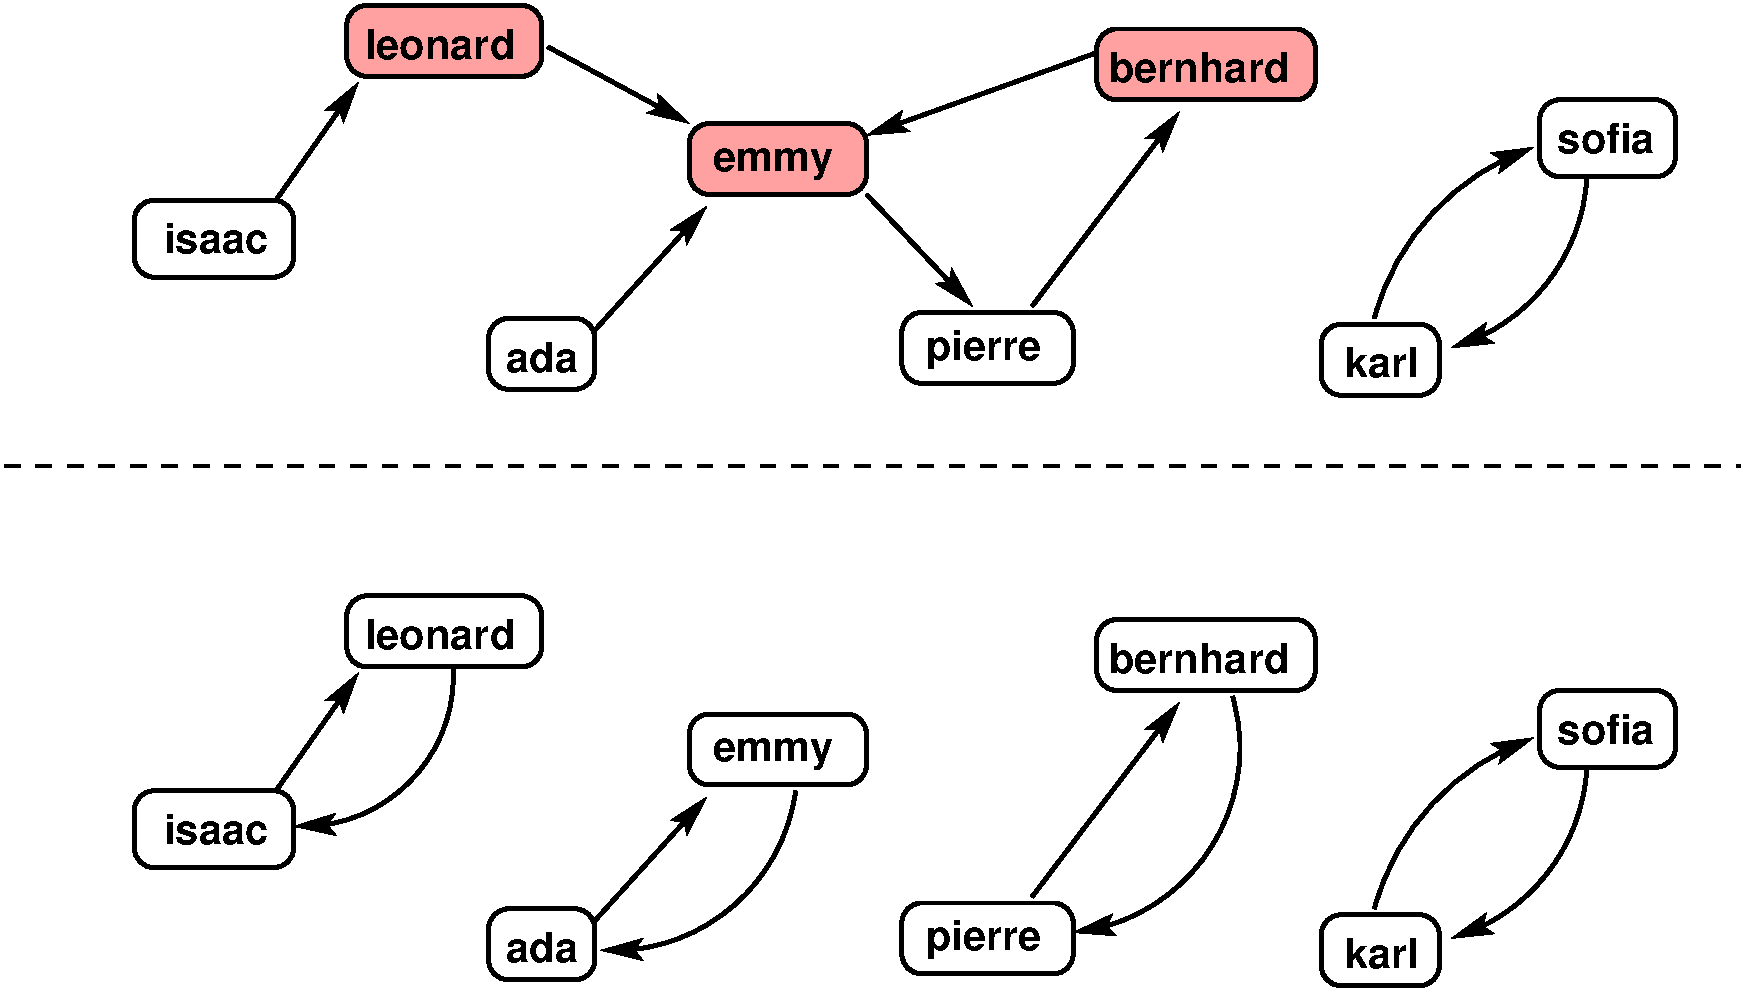
\includegraphics[width=0.5\textwidth]{polygonfig.pdf}
\end{center}

Pirmasis pavyzdys pavaizduotas paveikslėlyje aukščiau. Viršutinėje dalyje pavaizduota pradinė situacija, kur strėlė, vedanti iš $s$ į $t$, reiškia, kad pradiniu momentu $s$ įsimylėjęs $t$. Rožinė spalva parodo tris dalyvius, į kuriuos reikia paleisti strėles, norint gauti vienintelį optimalų sprendinį. Apatinėje dalyje pavaizduota situacija iššovus strėles.

Antrajame pavyzdyje (kuris tenkina 3-čios grupės ribojimus) galimi keli optimalūs sprendiniai.
Vienas jų yra paleisti strėles į  \texttt{a}, \texttt{b} ir \texttt{d}, kad jie įsimylėtų atitinkamai \texttt{b}, \texttt{a} ir \texttt{c}.

Trečiajame pavyzdyje yra meilės trikampis. Nesvarbu kaip ir kiek strėlių iššautume, vis viena liks kažkas, kas nebus užmezgęs santykių.

